\documentclass[a4paper,11pt]{article}

\usepackage{graphicx}
\usepackage{float}
\usepackage{listings}
\usepackage[colorlinks]{hyperref}
\title{OFBiz - Code Inspection}
\begin{document}

\begin{titlepage}
\begin{figure}
	\centering
	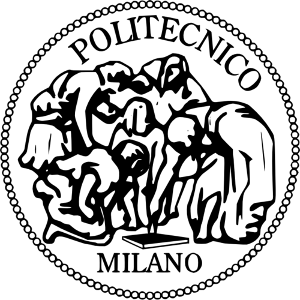
\includegraphics[width=0.5\textwidth]{images/polimi}
\end{figure}
\maketitle
\centering
A.Y. 2016/2017

Bolshakova Liubov, matr. 876911 

Gao Xiao, matr. 876265 

Kang Shuwen, matr. 876245

\end{titlepage}

\tableofcontents
\newpage
	
\section{CODE DESCRIPTION}
	\subsection{Assigned Classes}
	The assigned classes of our group are listed as follows:
	\subsubsection{RequirementServices.java}
	The class is located in: ../apache-ofbiz-16.11.01/applications/order/src
		/main/java/org/apache/ofbiz/order/requirement/RequirementServices.java
	\subsubsection{EntityEcaCondition.java}
	The class is located in: ../apache-ofbiz-16.11.01/framework/entityext/src
		/main/java/org/apache/ofbiz/entityext/eca/EntityEcaCondition.java
	\subsection{Introduction}
	\subsubsection{Apache OFBiz}
	Apache OFBiz is an open source enterprise resource planning (ERP) system. It provides a suite of enterprise applications that integrate and automate many of the business processes of an enterprise.
	
	All of Apache OFBiz functionality is built on a common framework. The functionality can be divided into the following distinct layers:
	\begin{itemize}
		\item \textbf{Presentation Layer}
		
		Apache OFBiz uses the concept of "screens" to represent the Apache OFBiz pages. 
		\item \textbf{Business Layer}
		
		The business, or application layer defines services provided to the user.
		\item \textbf{Data Layer}
		
		The data layer is responsible for database access, storage and providing a common data interface to the Business layer. 
	\end{itemize}
	\subsubsection{Order Manager}
	Order Manager is an application inside the OFBiz project, which is responded to due with the order processing. The Order Manager contains server sub-services, including:
	\begin{itemize}
		\item Main
		\item Requests
		\item Quotes
		\item Order List
		\item Find Orders
		\item Order Entry
		\item Returns
		\item Requirements
		\item Reports
		\item Stats
	\end{itemize}	
	\subsection{Functional Role of Classes}	
	\subsubsection{RequirementServices.java}
	One of our assigned classes, RequirementServices.java located in the business layer, is designed to provide the requirement service in the Order Manager application. As shown in Figures below, the requirement service provides four screens to search for requirements, which are
	\begin{itemize}
		\item \textbf{REQUIREMENTS}
		\item \textbf{APPROVE REQUIREMENTS}
		\item \textbf{FIND APPROVED REQUIREMENTS BY SUPPLIER}
		\item \textbf{APPROVED PRODUCT REQUIREMENTS}.
		\end{itemize}
		The requirement service also provides a screen named \textbf{New Requirement}, in order to manually add new requirement as well as edit existing requirement.
	
	\begin{figure}[H]
   			\centering
  			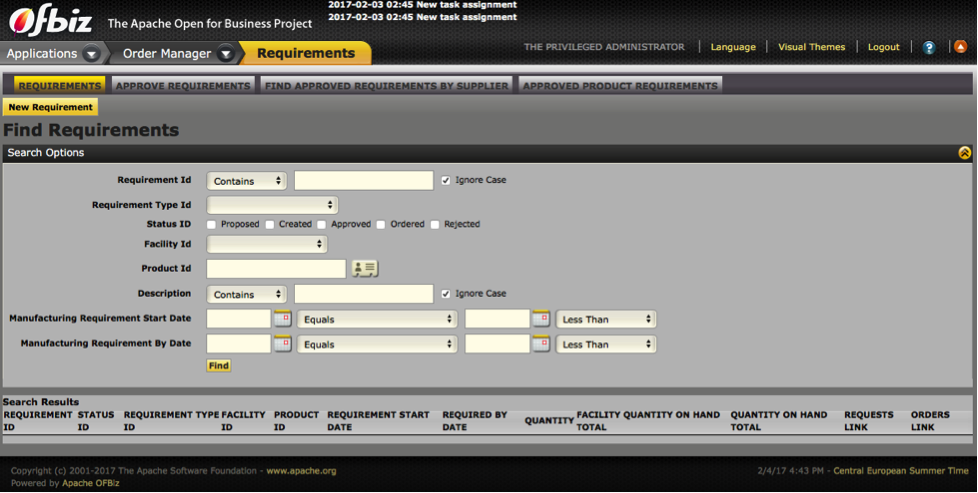
\includegraphics[width=\textwidth]{images/requirement}
  	    		\caption{REQUIREMENTS}\label{fig-req1}
		\end{figure}
	\begin{figure}[H]
   			\centering
  			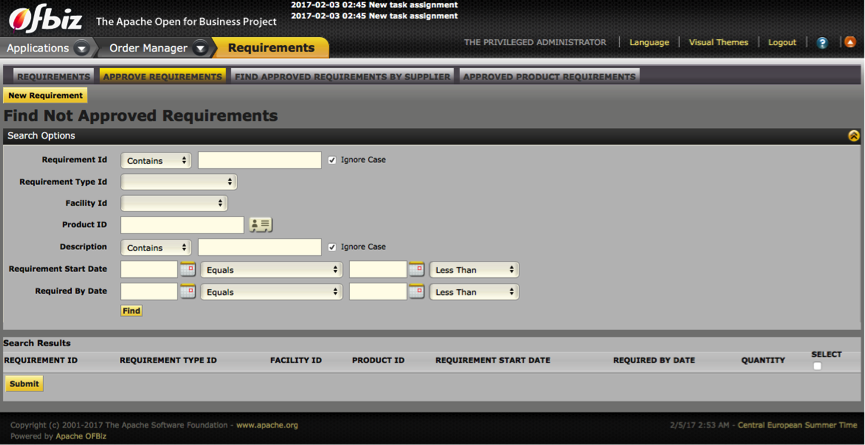
\includegraphics[width=\textwidth]{images/requirement2}
  	    		\caption{APPROVE REQUIREMENTS}\label{fig-req2}
		\end{figure}
	\begin{figure}[H]
   			\centering
  			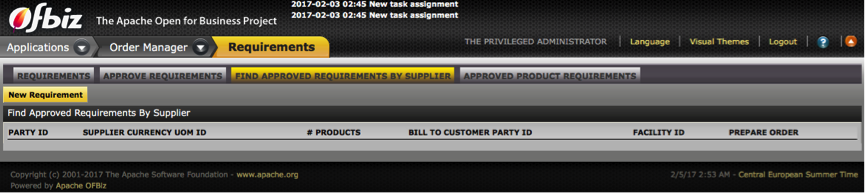
\includegraphics[width=\textwidth]{images/requirement3}
  	    		\caption{FIND APPROVED REQUIREMENTS BY SUPPLIER}\label{fig-req3}
		\end{figure}
	\begin{figure}[H]
   			\centering
  			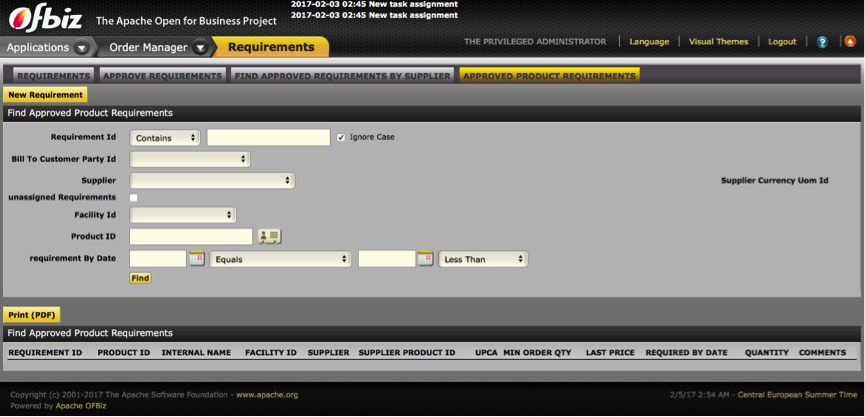
\includegraphics[width=\textwidth]{images/requirement4}
  	    		\caption{APPROVED PRODUCT REQUIREMENTS}\label{fig-req4}
		\end{figure}
	To achieve the business logic of functions displayed above, there are basically four methods in this class, and the particular functional role of each method is described in detail in the following paragraphs.
	\begin{itemize}
		\item \textbf{getRequirementsForSupplier()}
		
		This method preforms the most important role in the requirement service, by reading the searching condition, provided by the user, from the screen, and combining the condition into query, and finally return back the result from the database as a map to support the information presentation on the screen. Basically, this method provides the requirement searching result by either getting the requirements for a given supplier, unassigned requirements, or requirements for all suppliers.
		
		\item \textbf{createAutoRequirementsForOrder()}
		
		This method is designed to automatically create a requirement for an order, once a sales order status changes from CREATE to APPROVED.
		\item \textbf{createATPRequirementsForOrder()}
		
		The strategy in this service is to begin making requirements when the product falls below the ProductFacility.minimumStock.  Because the minimumStock is an upper bound, the quantity to be required is either that required to bring the ATP(Available to Promise) back up to the minimumStock level or the amount ordered, whichever is less.
         
         If there is a way to support reorderQuantity without losing the order item to requirement association data, then this service should be updated.
    
         The result is that this service generates many small requirements when stock levels are low for a product, which is perfectly fine since the system is capable of creating POs in bulk from aggregate requirements.
         The only concern would be a UI to manage numerous requirements with ease, preferrably by aggregating on productId.
		\item \textbf{updateRequirementsToOrdered()}
		
		This method is designed to change status of requirement to ORDERED. 
	\end{itemize}
	\subsubsection{EntityEcaCondition.java}
	There are basically six methods contained in this class, which are further discussed as follows.
	\begin{itemize}
	\item \textbf{eval()}
	
	This method is for check if the dispatch messages are sent out successfully , if it is successes,return right, else return false. This is the whole process of check a message. At first the method get the information about each dispatch, and check the basic information: if the order number, dctx and value exits,then get the satisfied name of dispatch, evaluate the condition and invoke the actions, then check if information in to message is in a specific format, finally check if any messages were returned send them out,only if all of them are correct, this dispatch process can be seen as successes.
	
	\item \textbf{getLValue()}
	
	This method is used by the eval() method, it returns the specific lhsValueName of the dispatch information.
	
	\item \textbf{getRValue()}
	
	This method is used by the eval() method, it returns the specific rhsValueName of the dispatch information.
	
	\item \textbf{getOperator()}
	
	This method is used by the eval() method, it returns the specific operator of the dispatch information.
	\item \textbf{toString()} 
	
This method is used by the eval() method for generating messages, it edits the information to the message and returns the message as a complete string.

	\item \textbf{getFieldNames()}
	
	This method is for generating a list of lhsValueName and rhsValueName which exist in the dispatch information and return this list as fieldNameList.
	\end{itemize}
	

	
\newpage
\section{INSPECTION RESULTS}
In this section, we present all the issues that we found during code inspection, according to the checklist provided by the Assignment. Notice that, the notation Point related to the check point numbered in the code inspection assignment document. 
	\subsection{Issues of RequirementServices.java}
	\subsubsection{Naming Conventions}
	\begin{itemize}
	\item \textbf{Point 7} 
	
	Two constant attributes of the class do not follow the naming convention for constants.
		\begin{itemize}
			\item module should be MODULE
			\item resource\_error should be RESOURCE\_ERROR
		\end{itemize}
	\end{itemize}
	\subsubsection{Indention}
	\begin{itemize}
	\item \textbf{Point 9} 
	
	Tabs are used to indent.
	\end{itemize}
	\subsubsection{Braces}
	\begin{itemize}
	\item \textbf{Point 11} 
	
	For the following lines, the single statement to execute is not surrounded by curly braces.
	\begin{itemize}
	\item Line 133
	\item Line 173
	\end{itemize}
	\end{itemize}
	\subsubsection{File Organization}
	\begin{itemize}
	\item \textbf{Point 13} 
	
	Many lines of code are not broken up properly and exceed 80 characters.
	\item \textbf{Point 14} 
	
	For the following lines, the line length exceed 120 characters.
	\begin{itemize}
		\item Line 130
		\item Line 162
		\item Line 225
		\item Line 230
		\item Line 285
		\item Line 292
		\item Line 318
		\item Line 320
	\end{itemize}
	\end{itemize}
	\subsubsection{Wrapping Lines}
	\begin{itemize}
	\item \textbf{Point 16} 
	
	Higher-level breaks are not used.
	\end{itemize}
	\subsubsection{Java Source Files}
	\begin{itemize}
	\item \textbf{Point 23} 
	
	The javadoc is not complete, and is missing for the following methods:
	\begin{itemize}
		\item getRequirementsForSupplier()
		\item createAutoRequirementsForOrder()
		\item createATPRequirementsForOrder()
		\item updateRequirementsToOrdered()
	\end{itemize}
	\end{itemize}
	\subsubsection{Output Format}
	\begin{itemize}
	\item \textbf{Point 42} 
	
	The following lines contain log error messages that do not provide guidance or hints on how to correct the problem:
	\begin{itemize}
	\item Line 235
	\item Line 237
	\item Line 325
	\item Line 327
	\item Line 352
	\item Line 354
	\end{itemize}
	\end{itemize}
	
	\subsection{Issues of EntityEcaCondition.java}
	\subsubsection{Indention}
	\begin{itemize}
	\item \textbf{Point 9} 
	
	Tabs are used to indent.
	\end{itemize}
	
	\subsubsection{Braces}
	\begin{itemize}
	\item \textbf{Point 11} 
	
	For the following lines, the single statement to execute is not surrounded by curly braces.
	\begin{itemize}
	\item Line 65
	\end{itemize}
	\end{itemize}
	
	\subsubsection{File Organization}
	\begin{itemize}
	\item \textbf{Point 13} 
	
	Many lines of code are not broken up properly and exceed 80 characters.
	\item \textbf{Point 14} 
	
	For the following lines, the line length exceed 120 characters.
	\begin{itemize}
		\item Line 76
		\item Line 80
		
	\end{itemize}
	\end{itemize}
	
	\subsubsection{Wrapping Lines}
	\begin{itemize}
	\item \textbf{Point 16} 
	
	Higher-level breaks are not used.
	\end{itemize}
	
	\subsubsection{Java Source Files}
	\begin{itemize}
	\item \textbf{Point 23} 
	
	The javadoc is not complete, and is missing for the following methods:
	\begin{itemize}
		\item getLValue()
		\item getRValue()
		\item getOperator()
		\item getFieldNames()
	\end{itemize}
	\end{itemize}

	
\newpage	
\section{APPENDIX}

		\subsection{Software and Tools Used}
The tools used to creat this document are:
	\begin{itemize}
		\item Github: for version control
		\item Latex: for typesetting
		 
	\end{itemize}

		\subsection{Hours of Work}
\renewcommand\arraystretch{2}
\begin{tabular}{| p{5cm}| p{7cm}|}
 \hline
Gao Xiao& 6 Hours \\
 \hline
Kang Shuwen& 6 Hours \\
 \hline
Liubov Bolshakova& 4 Hours \\
 \hline

\end{tabular}
		
\newpage
\section{REFERENCES}
\begin{itemize}
\item AA 2016/2017 Software Engineering 2 - Project goal, schedule and rules
\item AA 2016/2017 Software Engineering 2 - Code Inspection Assignment -
Task Description
\item OFBiz - Apache OFBiz Documentation
\item Apache OFBiz Project Open Wiki article
\item Wikipedia article on OFBiz \url{https://en.wikipedia.org/wiki/ Apache_OFBiz}

\end{itemize}

\newpage
	
\end{document}